% DriftLens -- IEEE conference format (IEEEtran), 6 pages
% Compile: pdflatex driftlens_ieee && bibtex driftlens_ieee && pdflatex driftlens_ieee && pdflatex driftlens_ieee
\documentclass[conference]{IEEEtran}

\usepackage{cite}
\usepackage{amsmath,amssymb}
\usepackage{graphicx}
\usepackage{booktabs}
\usepackage{tikz}
\usetikzlibrary{arrows.meta,positioning}
\usepackage{url}

\graphicspath{{../results/figures/}}
\newcommand{\state}[1]{\textsc{#1}}

\begin{document}

\title{DriftLens: Reading a Social-Media Timeline as a Sentence to Detect Moments of Change with Classical NLP}

% Replace [email] with the co-authors' addresses.
\author{\IEEEauthorblockN{B Varun}
\IEEEauthorblockA{Vellore Institute of Technology\\
Vellore, India\\
varun452005@gmail.com}
\and
\IEEEauthorblockN{Sagnik Basu}
\IEEEauthorblockA{Vellore Institute of Technology\\
Vellore, India\\
{[email]}}
\and
\IEEEauthorblockN{Arivoli A}
\IEEEauthorblockA{Vellore Institute of Technology\\
Vellore, India\\
{[email]}}}

\maketitle

\begin{abstract}
People who write about their mental health online rarely change in one step: some posts mark a sudden shift in mood, others belong to a slow slide or recovery. We ask how far the classical NLP toolkit can go in finding these moments of change, without large language models. DriftLens reads a user's timeline the way a part-of-speech tagger reads a sentence. Each post receives a hidden state (no change, switch, escalation, or both) decoded with hidden Markov models or conditional random fields, over evidence from components we build and evaluate one by one: a noisy-channel spelling corrector, a WordNet-grown self-state lexicon with adapted Lesk disambiguation, an HMM tagger feeding a grammar for self-evaluative statements, and a personal language-model novelty score. On 30 labelled CLPsych timelines (373 posts), sequence models reach a macro-F1 of 0.567 against 0.266 for the majority baseline and detect escalation better than a per-post maximum-entropy classifier. Post length alone already gives 0.572; within posts of similar length, however, the linguistic features add 0.09 to 0.13 macro-F1. The lexicon tracks annotated well-being better than VADER (Spearman 0.43 vs.\ 0.36) and, without training labels, separates depressed from control users in eRisk 2026 with an AUC of 0.84.
\end{abstract}

\begin{IEEEkeywords}
moments of change, sequence labelling, hidden Markov models, conditional random fields, WordNet, n-gram language models, mental health
\end{IEEEkeywords}

%======================================================================
\section{Introduction}
%======================================================================

Many people describe their emotional lives on public forums long before, or instead of, speaking to a clinician. A clinician reading such a history cares less about a single label for the person than about its turning points: the week the tone suddenly darkened, or the run of posts in which things slowly got worse. Tsakalidis et al.~\cite{tsakalidis2022identifying} turned this into a task. Given a chronological timeline of one user's Reddit posts, a system marks each post as a \emph{switch} (an abrupt change relative to the user's recent state), part of an \emph{escalation} (a gradual progression), or neither. The CLPsych 2022 shared task~\cite{tsakalidis2022overview} used this definition, and CLPsych 2025~\cite{tseriotou2025overview} added well-being ratings and evidence of adaptive and maladaptive self-states to the same kind of timelines.

Recent systems for the task usually encode posts with pre-trained transformers or prompt large language models; earlier work by one of us followed that path with an LLM teacher, judge and student~\cite{kumar2026triage}. Such models can be accurate but are costly and hard to inspect. We ask a narrower question: \emph{with only classical, textbook NLP methods~\cite{jurafsky2024speech}, which signals of change can be found, and which survive a careful evaluation?}

Two properties of the data make this sensible. A timeline is a sequence, much like a sentence: in the CLPsych training data, escalation labels come in 23 runs averaging 3.3 posts, exactly the structure an HMM transition matrix can hold. And a switch is defined relative to the person, which suggests measuring each post against the writer's own history. Our contributions are:
\begin{itemize}
\item moment-of-change detection cast as sequence labelling, with a MaxEnt classifier, a Gaussian HMM, a MaxEnt--HMM hybrid and a linear-chain CRF compared on identical features, plus a tuning-free prior-corrected decoding rule for class imbalance;
\item a \emph{personal language-model novelty} score and per-user standardised versions of every signal;
\item a self-state lexicon grown from 94 sense-specific WordNet seeds, filtered by a sense-ratio prior and a polarity veto, and validated on well-being ratings, evidence spans and an external depression corpus;
\item an error analysis exposing a strong post-length shortcut and showing, through ablations and length-stratified evaluation, where language still helps; and a CPU-only prototype exposing every component.
\end{itemize}

%======================================================================
\section{Related Work}
%======================================================================

\emph{Language and mental health.} Depressed writers use the first-person singular more often~\cite{rude2004language}, a finding built into dictionary tools such as LIWC~\cite{tausczik2010psychological}. Social-media text carries measurable signals of depression~\cite{dechoudhury2013predicting,coppersmith2014quantifying}, though many studies predict a static user-level label with weak construct validity~\cite{chancellor2020methods}. The eRisk campaign studies early depression detection from a user's writings~\cite{losada2016test,parapar2024erisk}.

\emph{Moments of change.} Tsakalidis et al.~\cite{tsakalidis2022identifying} introduced switch and escalation annotations and compared isolated-post models with models that see surrounding posts; many CLPsych 2022 systems built on transformer post representations~\cite{tsakalidis2022overview}. CLPsych 2025~\cite{tseriotou2025overview}, the release we use, turned to well-being scores, evidence extraction and summaries.

\emph{Sequence labelling and language change.} HMMs with Viterbi decoding~\cite{rabiner1989tutorial,viterbi1967error} are the textbook POS-tagging solution~\cite{brants2000tnt}; maximum-entropy models~\cite{berger1996maximum} and CRFs~\cite{lafferty2001conditional} are their conditional counterparts, and classifier posteriors can replace HMM emissions~\cite{bourlard1994connectionist}. Danescu-Niculescu-Mizil et al.~\cite{danescu2013no} measured linguistic change by cross-entropy against community language models; we apply the idea to a single user's history.

\emph{Lexicons from WordNet.} Hu and Liu~\cite{hu2004mining} grew opinion lexicons along WordNet synonyms and antonyms, SentiWordNet~\cite{esuli2006sentiwordnet} scores every synset, and VADER~\cite{hutto2014vader} is a hand-built social-media lexicon. Our seeds are senses rather than words, expanded words are weighted by how much of their usage falls in the reached senses, and we disambiguate with adapted Lesk~\cite{lesk1986automatic,banerjee2002adapted} plus a domain cue~\cite{magnini2002role}.

%======================================================================
\section{Data}
%======================================================================

\emph{CLPsych timelines.} The 30 labelled CLPsych 2025 training timelines contain 373 Reddit posts (5--25 per timeline, median 44 words). Each post has a switch and an escalation flag; 236 posts also carry a 1--10 well-being rating with evidence spans (615 maladaptive, 472 adaptive). Since the flags co-occur we use four states: \state{O} (no change, 66.2\%), \state{S} (switch, 13.7\%), \state{E} (escalation, 12.9\%) and \state{B} (both, 7.2\%). The 10 test timelines are unlabelled, so supervised results use cross-validation and the test timelines appear only in the prototype.

\emph{eRisk 2026.} Task~2~\cite{erisk2026} has 909 users (102 depressed). Keeping only each target user's own writings, a 1.5M-token sample trains the background language model, and user labels give an external test of the lexicon (which does not use the language model).

\emph{Other resources and ethics.} The tagger is trained on the Brown corpus~\cite{francis1979brown} with universal tags~\cite{petrov2012universal}; the spelling dictionary joins Brown, the NLTK word list and WordNet~\cite{miller1995wordnet} lemmas. Both mental-health corpora are under data-use agreements: all processing is local, no post is quoted here, and example sentences are our own~\cite{benton2017ethical}.

%======================================================================
\section{Method}
%======================================================================

\begin{figure*}[t]
\centering
\resizebox{0.92\textwidth}{!}{%
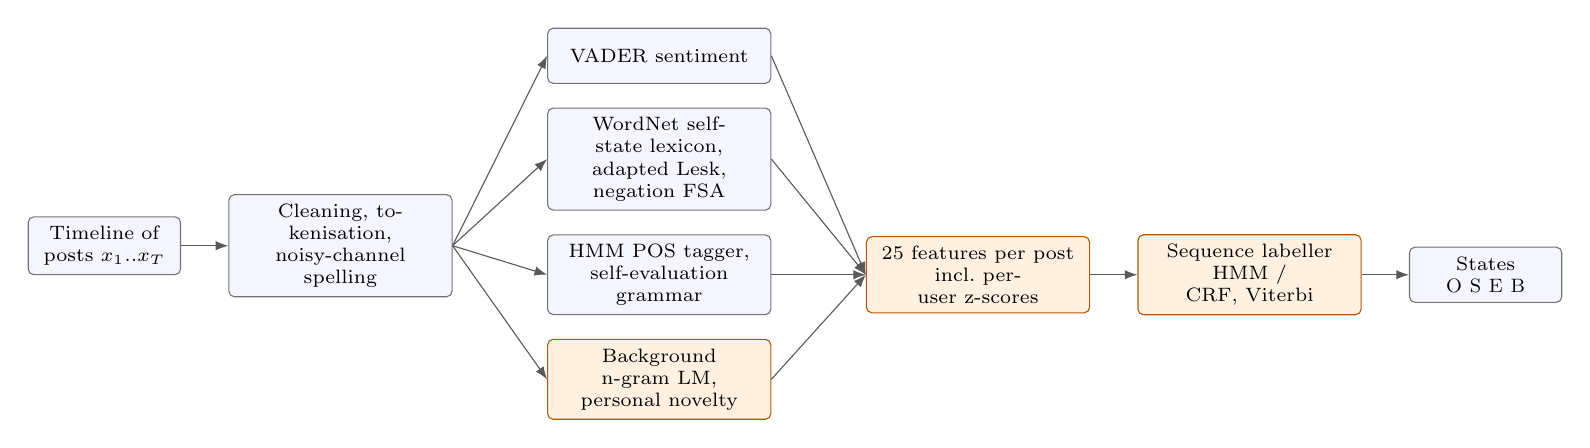
\begin{tikzpicture}[
  node distance=3mm and 6mm,
  box/.style={draw=black!55, rounded corners=2pt, align=center, font=\scriptsize, fill=blue!4, minimum height=7mm, text width=26mm},
  hl/.style={box, fill=orange!12, draw=orange!70!black},
  arr/.style={-{Latex[length=1.6mm]}, draw=black!65}]
  \node[box, text width=17mm] (in) {Timeline of\\posts $x_1..x_T$};
  \node[box, right=of in] (norm) {Cleaning, tokenisation,\\noisy-channel spelling};
  \node[box, right=12mm of norm, yshift=11mm] (lex) {WordNet self-state lexicon,\\adapted Lesk, negation FSA};
  \node[box, below=of lex] (pos) {HMM POS tagger,\\self-evaluation grammar};
  \node[hl, below=of pos] (lm) {Background n-gram LM,\\personal novelty};
  \node[box, above=of lex] (vad) {VADER sentiment};
  \node[hl, right=12mm of pos] (feat) {25 features per post\\incl.\ per-user z-scores};
  \node[hl, right=of feat] (seq) {Sequence labeller\\HMM / CRF, Viterbi};
  \node[box, right=of seq, text width=17mm] (out) {States\\\state{O} \state{S} \state{E} \state{B}};
  \draw[arr] (in) -- (norm);
  \foreach \t in {lex,pos,lm,vad} \draw[arr] (norm.east) -- (\t.west);
  \foreach \t in {lex,pos,lm,vad} \draw[arr] (\t.east) -- (feat.west);
  \draw[arr] (feat) -- (seq);
  \draw[arr] (seq) -- (out);
\end{tikzpicture}}
\caption{The DriftLens pipeline. Every component is a classical, CPU-only NLP method; orange boxes model change relative to the user and over time. Only the sequence labeller sees CLPsych labels.}
\label{fig:pipeline}
\end{figure*}

Fig.~\ref{fig:pipeline} shows the pipeline. Four label-free components score each post; their outputs form a feature vector and a sequence model assigns the states. Because nothing before the sequence model sees a label, features are computed once, outside cross-validation.

\subsection{Noisy-Channel Spelling Correction}
Reddit markup is removed, letters repeated three or more times are shortened to two, apostrophe-less contractions (\emph{im}, \emph{dont}) are expanded, and text is segmented with NLTK's Punkt and Treebank tokenisers. For a token $x$ outside the dictionary (after WordNet's inflectional analysis) the corrector picks
\begin{equation}
\begin{split}
\hat{w} = \arg\max_{w \in C(x) \cup \{x\}} \; & \log P(w \mid w_{-1}) + \log P(w_{+1} \mid w) \\
& - \alpha\, d(x, w),
\end{split}
\end{equation}
with $C(x)$ the dictionary words within two edits and bigram probabilities from the background model (Sect.~\ref{sec:lm}); out-of-vocabulary candidates share the \texttt{<unk>} mass in proportion to unigram counts. The channel $d$ is a weighted Damerau--Levenshtein distance~\cite{damerau1964technique,kernighan1990spelling}: 0.5 for adjacent QWERTY keys, 0.7 for vowel swaps, 0.6 for doubled-letter edits and transpositions, 1 otherwise. Keeping $x$ itself ($d=0$) is the ``no error'' hypothesis that lets slang and names survive.

\subsection{Background LM and Personal Novelty}
\label{sec:lm}
The background model is a word bigram model with Jelinek--Mercer interpolation~\cite{jelinek1980interpolated,chen1999empirical}, $P_{\text{bg}} = \lambda_2 P_{\text{ML}}(w_i \mid w_{i-1}) + \lambda_1 P_{\text{add-}k}(w_i)$, trained on 1.5M eRisk tokens with $\lambda$ tuned on 60k held-out tokens. For post $t$ we train an add-$k$ bigram model $P_{u,t}$ ($k=0.05$) on the same user's posts $1..t-1$, mix $P_{\text{mix}} = \beta P_{u,t} + (1-\beta) P_{\text{bg}}$ with $\beta = 0.3$, and define novelty as the change in cross-entropy (bits per token):
\begin{equation}
\mathrm{nov}_t = H_{\text{mix}}(x_t) - H_{\text{bg}}(x_t).
\end{equation}
A post that reuses the writer's habitual phrasing gets negative novelty; one that breaks from it approaches the bound $-\log_2(1-\beta) \approx 0.51$. Subtracting $H_{\text{bg}}$ removes how predictable the text is in general. We also record the share of content words new to the user.

\subsection{WordNet-Grown Self-State Lexicon}
Twelve categories follow the CLPsych 2025 self-state evidence: seven maladaptive (despair, self-criticism, anxiety, anger, isolation, exhaustion, crisis) and five adaptive (hope, connection, calm, joy, agency). The 94 seeds are synsets, so the emotional sense of \emph{hopeless} is kept apart from ``hopeless at maths''. From each seed we follow similar-to, also-see, attribute, derivation, pertainym, verb-group and hyponym links for two hops, multiplying the weight by 0.7--0.85 per hop; hyponyms must stay within Wu--Palmer similarity~\cite{wu1994verb} 0.6 of the seed, crisis seeds admit only derivations, and antonyms seed the opposite polarity with weight 0.6. A reached word may still be used mostly in another sense, so we compute its \emph{sense ratio}
\begin{equation}
r(w) = \frac{\sum_{s \in S_{\text{reached}}(w)} (c(w,s)+1)}{\sum_{s \in S(w)} (c(w,s)+1)},
\end{equation}
where $S(w)$ holds the synsets listing $w$ as a lemma and $c$ is the SemCor count. Weights are scaled by $\sqrt{r(w)}$ and words with $r(w) < 0.2$ are dropped, removing \emph{down}, \emph{blue} and \emph{low}. Expanded words whose SentiWordNet~\cite{esuli2006sentiwordnet} or VADER polarity contradicts their category are vetoed. The result has 1,760 words (1,076 maladaptive, 684 adaptive) after 312 vetoes, plus 30 hand-written multi-word expressions (\emph{end it all}, \emph{reach out}).

At scoring time a token is looked up directly, after WordNet's \texttt{morphy}, and after a derivational suffix stripper (\emph{hopelessness} $\rightarrow$ \emph{hopeless}). The 700 words with $r(w) < 0.7$ are disambiguated by adapted Lesk~\cite{banerjee2002adapted}: a sense's signature pools the content words of its gloss, examples and lemmas and those of its neighbours; lexicon senses gain a point when another affect word shares the sentence~\cite{magnini2002role}; ties go to the more frequent sense. A hit counts only for a reached sense, so ``anxious to see the new film'' is rejected. A two-state finite-state machine handles negation: a cue opens a three-word scope closed by clause boundaries; a negated adaptive word counts half towards maladaptive (``not happy''), and a negated maladaptive word is dropped.

\subsection{HMM Tagger and Self-Evaluation Grammar}
A bigram HMM over the 12 universal tags is trained on 51,606 Brown sentences (add-$k$ smoothing) and decoded with Viterbi; unknown words use TnT-style suffix distributions~\cite{brants2000tnt}. First-person pronouns, copulas, auxiliaries and negations are then re-tagged and a cascaded regular grammar, a finite-state approximation of a small CFG, chunks clauses such as ``I am so worthless'', ``I don't enjoy'' and ``I hate myself''. A chunk is a negative or positive self-evaluation according to the lexicon polarity of its words, with internal negation flipping adaptive words.

\subsection{Features and Sequence Models}
Table~\ref{tab:features} lists the 25 features. Deltas to the next post are allowed because the task is retrospective. The PERS group re-expresses six signals as z-scores within the user's own timeline.

\begin{table}[t]
\caption{Per-post features (balance = adaptive $-$ maladaptive score)}
\label{tab:features}
\centering\footnotesize
\begin{tabular}{@{}lcp{0.70\columnwidth}@{}}
\toprule
Group & \# & Features \\
\midrule
LEN & 1 & log word count \\
LEX & 8 & maladaptive, adaptive, balance, crisis; balance vs.\ running mean, previous and next post; $|$deviation from mean$|$ \\
SENT & 3 & VADER compound; change from previous, to next post \\
SELF & 3 & first-person rate; negative, positive self-evaluations \\
DRIFT & 2 & personal LM novelty; share of new content words \\
TIME & 2 & log days since previous post; first-post flag \\
PERS & 6 & within-user z-scores of length, maladaptive, balance, VADER, first person, novelty \\
\bottomrule
\end{tabular}
\end{table}

With $\mathbf{x}_{1:T}$ the feature vectors and $y_t \in \{\state{O},\state{S},\state{E},\state{B}\}$, we compare four families that mirror the classical POS-tagging models. \emph{MaxEnt} is class-balanced multinomial logistic regression~\cite{berger1996maximum} labelling posts independently. The \emph{Gaussian HMM} is estimated by supervised maximum likelihood with add-one transitions and diagonal-Gaussian emissions, and decoded by Viterbi:
\begin{equation}
\hat{y}_{1:T} = \arg\max_{y_{1:T}} \log \pi_{y_1} + \sum_{t=2}^{T} \log A_{y_{t-1} y_t} + \sum_{t=1}^{T} \log p(\mathbf{x}_t \mid y_t).
\end{equation}
The \emph{MaxEnt--HMM hybrid} replaces emissions with scaled likelihoods~\cite{bourlard1994connectionist}, either $p(y \mid \mathbf{x})/p(y)$ (prior-divided) or the posterior of a class-balanced classifier (balanced). The \emph{linear-chain CRF}~\cite{lafferty2001conditional} is trained with L-BFGS and $c_1 = c_2 = 0.1$ in CRFsuite~\cite{okazaki2007crfsuite}. Since Viterbi decoding of a likelihood-trained CRF favours the majority state, we also use \emph{prior-corrected posterior decoding}, $\hat{y}_t = \arg\max_y P(y_t = y \mid \mathbf{x}_{1:T}) / \pi^{\text{train}}_y$, the Bayes decision under a uniform state prior.

%======================================================================
\section{Experimental Setup}
%======================================================================

All supervised results use five-fold cross-validation at the \emph{timeline} level, repeated with five shuffles; out-of-fold predictions are pooled and we report mean $\pm$ standard deviation over repetitions. We score three binary views, switch (\state{S}/\state{B}), escalation (\state{E}/\state{B}) and no change, and macro-F1 is their mean F1. Hyper-parameters are library defaults fixed in advance, as 30 timelines are too few for nested tuning. Significance uses a paired bootstrap over timelines~\cite{bergkirkpatrick2012empirical} (1,000 resamples, metric averaged over repetitions). The class-balance corrections and personal z-scores were added after a first cross-validation run; earlier variants are reported alongside, and as no untouched labelled test set exists, numbers may be slightly optimistic.

%======================================================================
\section{Results}
%======================================================================

\subsection{Components on Their Own}

\begin{table}[t]
\caption{Component evaluation. Perplexity on all 465 CLPsych posts (LMs trained on 1.5M eRisk tokens); universal-tag accuracy (\%); spelling top-1 accuracy (\%) on 1,000 synthetic non-word errors}
\label{tab:components}
\centering\footnotesize
\begin{tabular}{@{}lr@{\hspace{10pt}}lr@{}}
\toprule
Language model & PPL & Tagger / speller & Acc. \\
\midrule
1-gram, Laplace & 604 & HMM, ours (Brown) & \textbf{96.9} \\
2-gram, Laplace & 1,335 & HMM, ours (Treebank) & 88.9 \\
2-gram, add-$k$ & 276 & NLTK perceptron (Brown) & 92.0 \\
2-gram, Jelinek--Mercer & 192 & NLTK perceptron (Treebank) & 96.1 \\
3-gram, Laplace & 10,541 & Levenshtein + unigram & 88.8 \\
3-gram, add-$k$ & 1,629 & Weighted + unigram & 90.7 \\
3-gram, Jelinek--Mercer & \textbf{176} & Weighted + bigram context & \textbf{95.3} \\
 & & \quad + ``no error'' option & 94.1 \\
\bottomrule
\end{tabular}
\end{table}

Table~\ref{tab:components} reproduces the classic smoothing lesson: add-one smoothing makes a trigram model worse than a unigram model (perplexity 10,541 vs.\ 604), while interpolation is best (176). Our HMM tagger reaches 96.9\% on held-out Brown text and 88.9\% on the Treebank sample; NLTK's perceptron, trained on Wall Street Journal text, shows the mirror image. For spelling, the keyboard-weighted channel helps most on adjacent-key substitutions (97\% vs.\ 90\%) and bigram context on deletions (84\% vs.\ 66--69\%). The ``no error'' option costs 1.2 points on synthetic errors but rewrites 63\% instead of 89\% of the 341 real out-of-dictionary CLPsych tokens, sparing slang and names.

\subsection{Is the Lexicon Measuring Self-State?}

\begin{figure}[t]
\centering
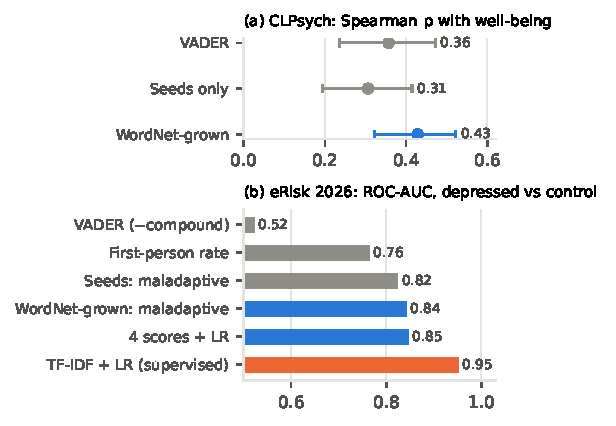
\includegraphics[width=\columnwidth]{fig_lexicon_ieee}
\caption{Lexicon validity. (a) Spearman correlation of the post balance score with annotated well-being (236 posts, 95\% bootstrap intervals). (b) ROC-AUC for 102 depressed vs.\ 807 control eRisk users (last 100 writings each); only the orange bar uses training labels.}
\label{fig:lexicon}
\end{figure}

On CLPsych (Fig.~\ref{fig:lexicon}a), the balance score correlates with well-being at $\rho = 0.43$ [0.32, 0.52], against 0.31 for seed lemmas and 0.36 for VADER; post length is unrelated ($\rho = -0.06$). The signal is maladaptive ($\rho = -0.47$); the adaptive score is flat ($-0.01$). The lexicon hits 39\% of the 615 maladaptive evidence spans (seeds: 31\%) at 38\% hit precision; adaptive evidence is harder (27\% recall, 25\% precision). On eRisk (Fig.~\ref{fig:lexicon}b), maladaptive density separates depressed from control users with AUC 0.84 and no labels; first-person rate gives 0.76, replicating~\cite{rude2004language}, while VADER is at chance (0.52). Depressed users use \emph{more} adaptive words (AUC 0.69), plausibly because they write in support communities. A supervised TF-IDF model is stronger (0.95), but cannot explain its evidence word by word. WSD, negation and spelling correction each moved $\rho$ by at most 0.012, so we do not claim they improve aggregate scores.

\subsection{Detecting Moments of Change}

\begin{table}[t]
\caption{Moment-of-change detection: 30 timelines, 373 posts, $5\times$5-fold timeline-level CV (mean $\pm$ s.d.)}
\label{tab:main}
\centering\footnotesize
\begin{tabular}{@{}lccc@{}}
\toprule
System & Macro-F1 & F1 sw. & F1 esc. \\
\midrule
Majority (all \state{O}) & 0.266 $\pm$ .000 & 0.000 & 0.000 \\
MaxEnt, post length only & \textbf{0.572} $\pm$ .008 & 0.483 & 0.470 \\
\midrule
MaxEnt (independent posts) & 0.547 $\pm$ .002 & 0.476 & 0.420 \\
Gaussian HMM & 0.567 $\pm$ .008 & \textbf{0.508} & 0.469 \\
Hybrid HMM, prior-divided & 0.542 $\pm$ .005 & 0.357 & 0.471 \\
Hybrid HMM, balanced & 0.532 $\pm$ .013 & 0.335 & 0.467 \\
CRF, Viterbi & 0.533 $\pm$ .011 & 0.374 & 0.416 \\
CRF, prior-corrected & 0.563 $\pm$ .008 & 0.472 & \textbf{0.481} \\
\bottomrule
\end{tabular}
\end{table}

Table~\ref{tab:main} gives the main results. All models are far above the majority baseline (HMM: bootstrap $p < 0.001$). The Gaussian HMM has the best full-feature macro-F1 (0.567) and switch F1 (0.508); the prior-corrected CRF has the best escalation F1 (0.481). Against per-post MaxEnt the HMM gains 0.049 escalation F1 ($p = 0.086$) and 0.032 switch F1 ($p = 0.087$), consistent across repetitions but not significant at 5\% with 30 timelines. Prior-corrected decoding lifts the CRF from 0.533 to 0.563 macro-F1 (switch F1 0.374 $\rightarrow$ 0.472). The learned HMM transitions explain the escalation gain: escalation persists ($\state{E}\!\to\!\state{E}$ 0.42, $\state{B}\!\to\!\state{E}$ 0.50), while a switch is usually followed by no change (0.65).

The second row matters most. Logistic regression on log post length alone reaches 0.572, and neither the HMM ($-0.006$, $p = 0.60$) nor the CRF ($-0.010$, $p = 0.67$) beats it. Change posts are much longer: about 150 words at the median versus 20 for unchanged posts (Mann--Whitney $p < 10^{-19}$). Length is a real signal, since people write at length when something has happened, but also a shortcut~\cite{geirhos2020shortcut}: a model relying on it misses a short, bleak post and flags every long, cheerful one.

\begin{table}[t]
\caption{Macro-F1 within length strata (median split at 46 words)}
\label{tab:strata}
\centering\footnotesize
\begin{tabular}{@{}lcc@{}}
\toprule
System & Short posts & Long posts \\
\midrule
MaxEnt, post length only & 0.311 & 0.369 \\
MaxEnt, all features & 0.393 & 0.463 \\
Gaussian HMM & 0.373 & 0.413 \\
CRF, prior-corrected & \textbf{0.404} & \textbf{0.495} \\
\bottomrule
\end{tabular}
\end{table}

Table~\ref{tab:strata} separates the effects. Within posts of similar length, the length model drops to 0.31 and 0.37, while the CRF with all features reaches 0.40 and 0.50, gains of 0.09 and 0.13. The overall tie hides a real contribution: length decides \emph{which half} of the data a post falls into, and the features decide which posts \emph{within} each half are moments of change. The HMM gains less, likely because its diagonal-Gaussian posteriors are very confident and mostly exploit the length split.

\subsection{What the Features Contribute}

\begin{figure}[t]
\centering
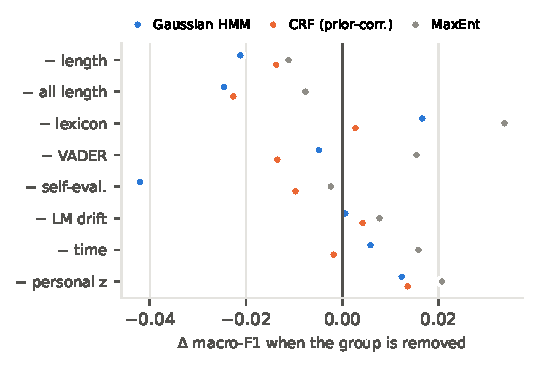
\includegraphics[width=\columnwidth]{fig_ablation_ieee}
\caption{Change in cross-validated macro-F1 when one feature group is removed (full: HMM 0.567, CRF 0.563, MaxEnt 0.547). Negative values mean the group helps.}
\label{fig:ablation}
\end{figure}

Fig.~\ref{fig:ablation} removes one group at a time. Self-evaluation chunks from the tagger and grammar are the most useful non-length group for the HMM ($-0.042$), and VADER helps the CRF ($-0.014$). Removing the lexicon group or the personal z-scores slightly \emph{improves} the models (up to $+0.034$): with 373 posts and 25 features, groups that repeat information (balance vs.\ VADER, z-scores vs.\ running-mean deltas) add variance. The lexicon still matters, since building features from seed lemmas lowers the HMM from 0.567 to 0.547, and user-relative signals carry much information alone (the PERS group reaches 0.533 with the HMM). The signals behave as expected: balance is lower for change posts (median $-0.91$ for \state{E} vs.\ 0.00 for \state{O}, $p < 10^{-4}$) and VADER separates the two kinds of change (switch posts +0.46, often sudden improvements; escalation posts $-0.68$). Personal LM novelty is the exception: higher for switch posts (0.26 vs.\ 0.21 bits) but not significantly different overall ($p = 0.25$); a bigram model of a dozen posts is too weak to show that a changing person sounds unlike themselves. Error analysis also shows long escalation runs labelled as series of switches, as pairwise deltas only approximate a trend.

%======================================================================
\section{Prototype}
%======================================================================

A Streamlit application runs the full pipeline on a laptop CPU, loading all models in under a second. Users paste their own posts or choose a CLPsych timeline; the main view plots balance, VADER and novelty with predicted and gold state bands, and each post shows highlighted maladaptive, adaptive, crisis and negated words, extracted self-evaluations, spelling corrections and state probabilities. An affect-biased TextRank digest~\cite{mihalcea2004textrank} summarises the timeline (not evaluated). A toolbox tab gives one interactive panel per technique: the noisy-channel candidate table, bigram probabilities and live novelty, HMM versus perceptron tags with chunk trees and top-down and bottom-up CFG parses, and WordNet similarity measures with both Lesk variants. We deploy the prior-corrected CRF, whose score is within noise of the HMM but whose probabilities are better calibrated.

%======================================================================
\section{Limitations and Ethics}
%======================================================================

The evaluation rests on 30 labelled timelines, so differences of 0.02 macro-F1 are noise, and some design choices followed a first cross-validation run. The lexicon categories and seeds are our reading of the CLPsych framework, and all data are English Reddit posts; code-mixed Hindi--English would need new resources at every stage. A system that labels mental states can harm people if it is wrong or misused. DriftLens is a research prototype, not a diagnostic or monitoring tool; it shows its evidence so a human can disagree, and displays the Indian Tele-MANAS helpline (14416).

%======================================================================
\section{Conclusion}
%======================================================================

Reading a timeline as a sentence works: HMMs and CRFs over classical features find moments of change far above chance, and sequence structure helps most where labels come in runs, on escalation. The more useful lesson concerns evaluation: post length alone matches every model, and only a length-stratified analysis reveals the 0.09--0.13 macro-F1 that language adds. A WordNet-grown lexicon also proved a better measure of self-state than a general sentiment tool, both on well-being ratings and, label-free, on an external depression corpus. Next steps are trend features over windows of posts and character-level personal language models.

\section*{Acknowledgment}
We thank the CLPsych and eRisk organisers for access to their data.

% balance the two columns on the last page
\IEEEtriggeratref{25}
\bibliographystyle{IEEEtran}
\bibliography{references}

\end{document}
